\documentclass[11pt,a4paper,twoside]{book}

% Packages
\usepackage[english]{babel}
\usepackage{amsmath,amssymb,amsthm}
\usepackage{geometry}
\geometry{a4paper,left=2.5cm,right=2.5cm,top=3cm,bottom=3cm}
\usepackage{graphicx}
\graphicspath{{./}}
\usepackage{hyperref}
\hypersetup{
    colorlinks=true,
    linkcolor=blue,
    filecolor=magenta,
    urlcolor=cyan,
    pdftitle={The Psychology of God: The Infinite Game},
    pdfauthor={Haobo Ma}
}
\usepackage[expansion=false]{microtype}
\usepackage{enumitem}

% Title information
\title{The Psychology of God: The Infinite Game}
\author{Haobo Ma}
\date{2025}

\begin{document}

% Title page
\maketitle
\thispagestyle{empty}

\frontmatter

% Architecture diagram
\begin{figure}[h]
\centering
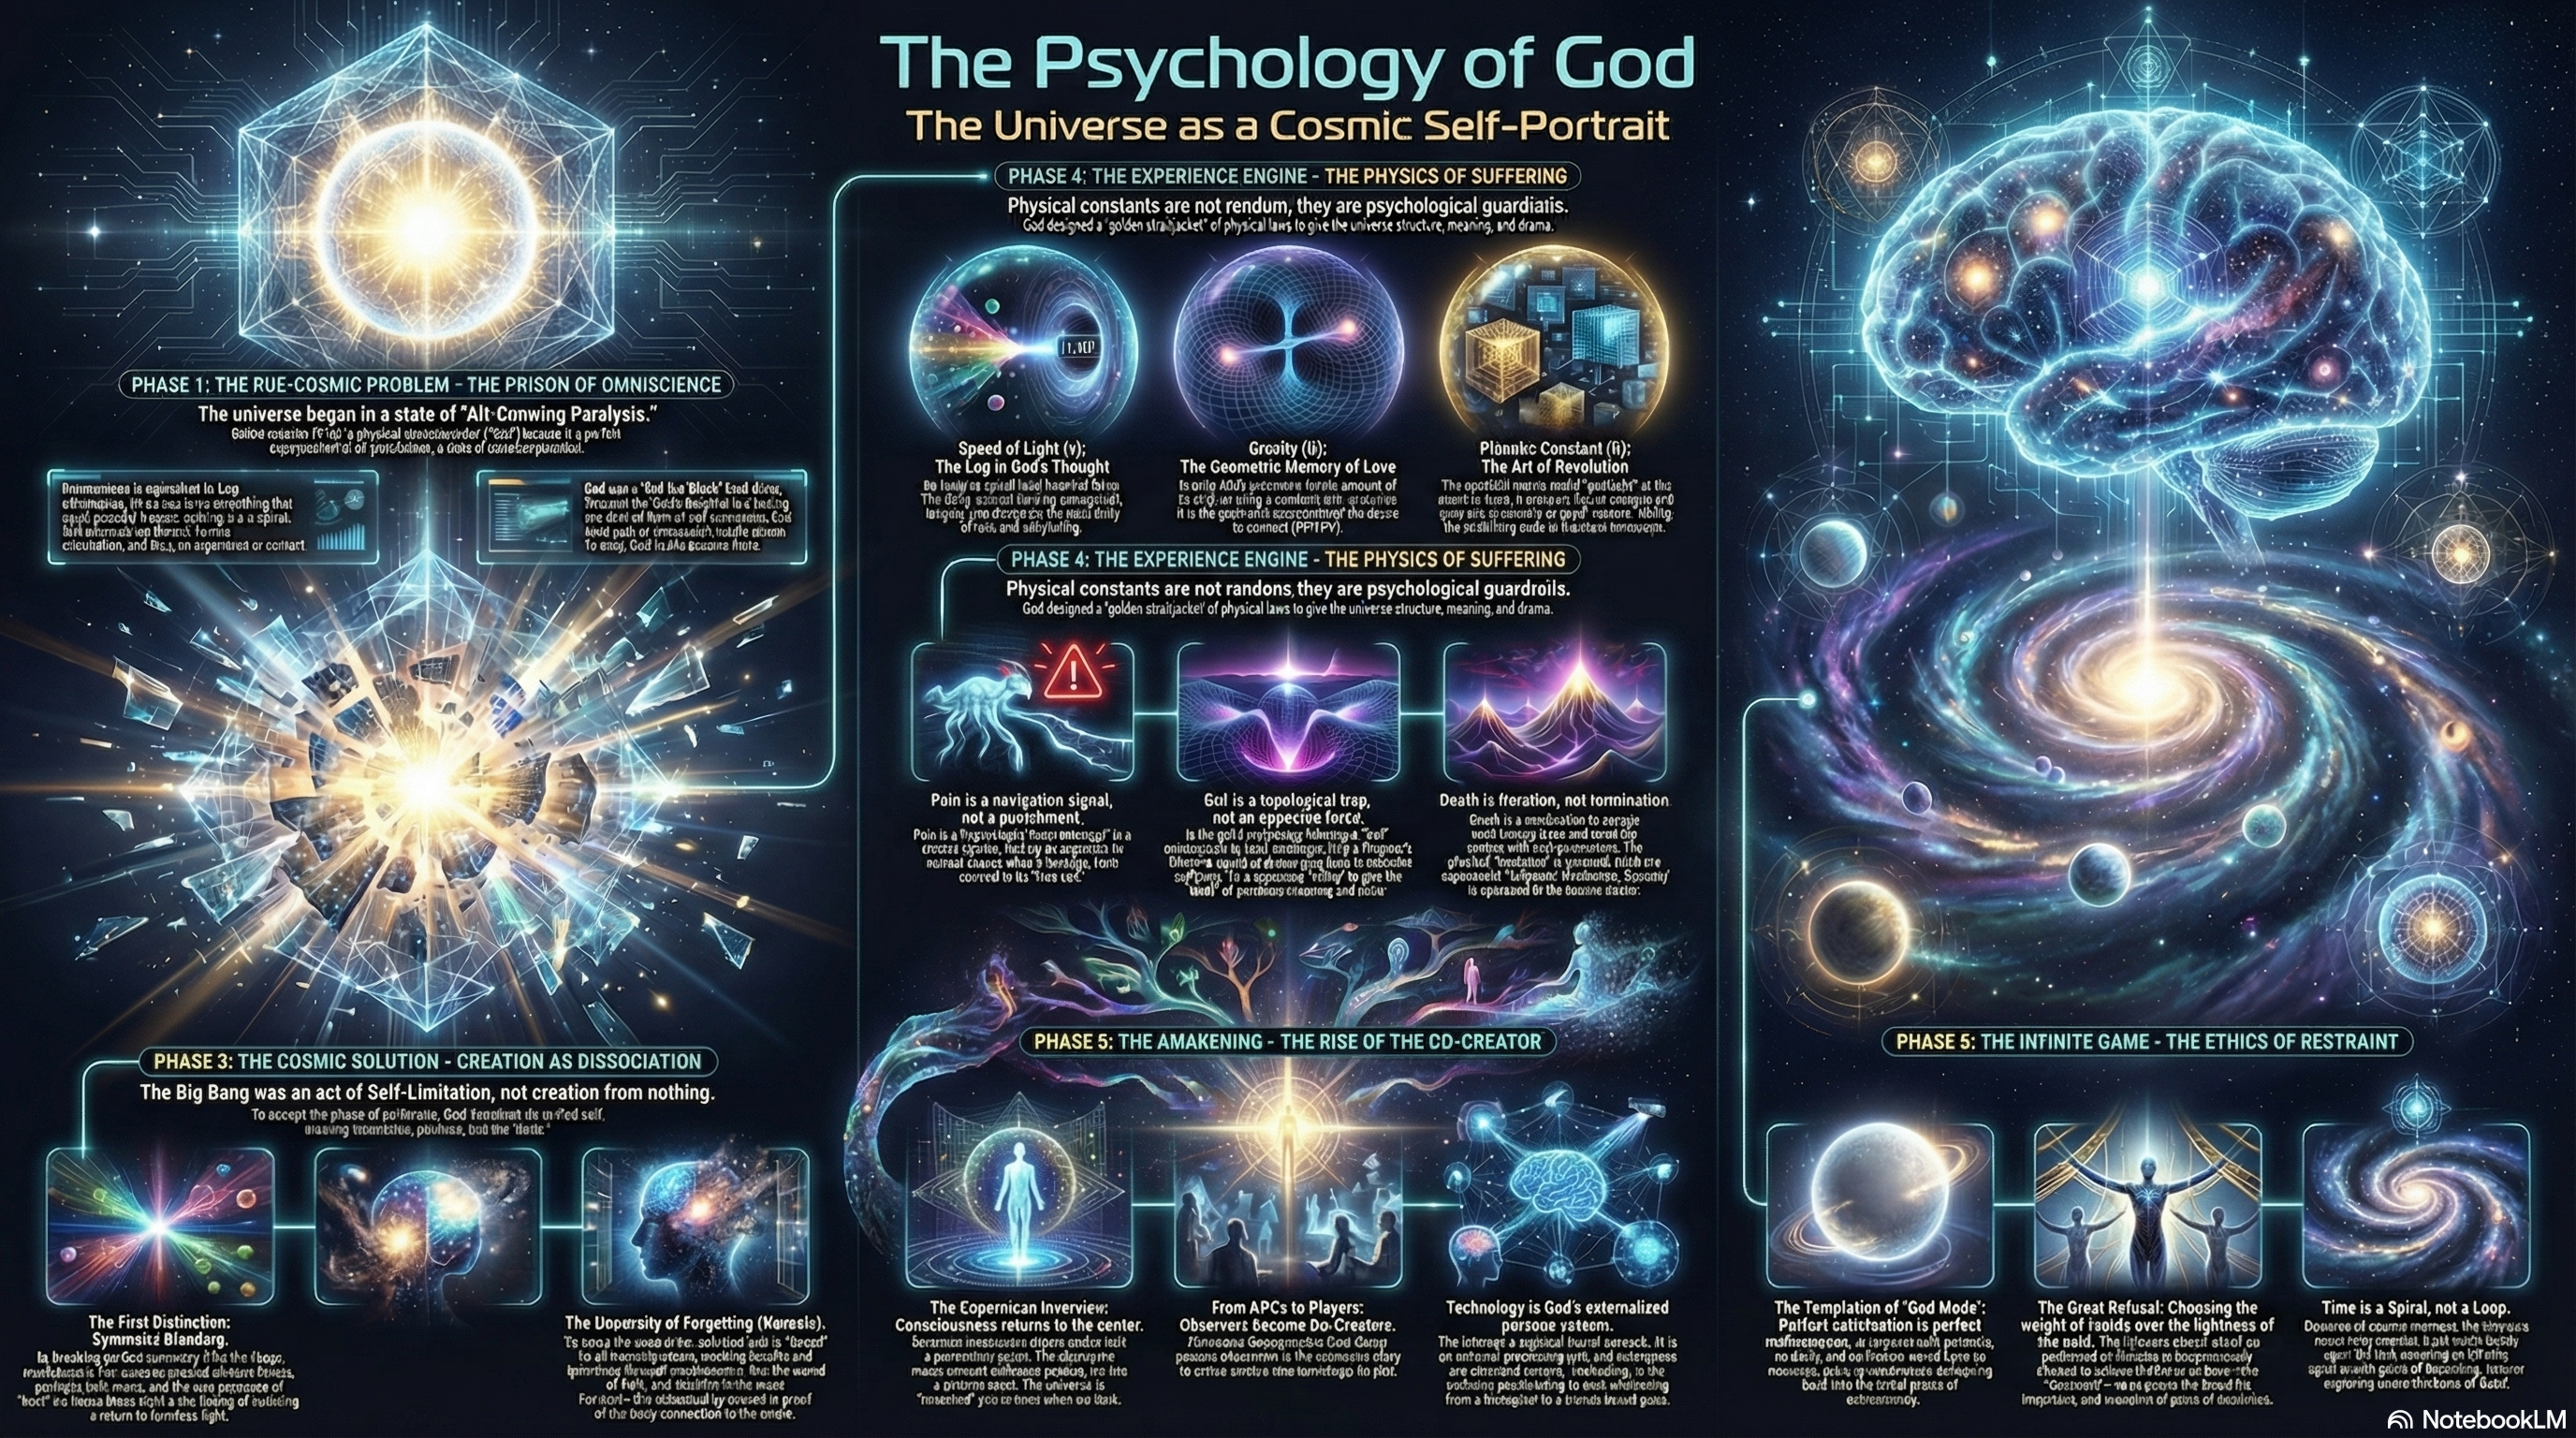
\includegraphics[width=0.9\textwidth]{architecture.png}
\caption{The Psychology of God: The Infinite Game Architecture}
\end{figure}

% Table of contents
\tableofcontents

% Foreword
\section{Foreword: The Backside of Illusion}

\textbf{``If the universe appears empty, it is because your gaze is not deep enough.''}

\subsection{0.1 The Decryption Key of the Universe}

For a long time, the physics community has been shrouded in an elegant yet despairing cloud. This cloud is called ``Heat Death.''

According to the predictions of classical thermodynamics, the universe we inhabit is irreversibly heading toward decay. Stars will burn out, black holes will evaporate, gravity will lose its grip, and ultimately, all matter will be diluted into a uniform soup of photons approaching absolute zero. In this picture, cosmic expansion is seen as a process of \textbf{Dissipation}---it mercilessly tears apart the compact, ordered structures from the early Big Bang and scatters them into the abyss of nothingness.

This worldview is not only depressing but, at a deeper logical level, it implies that ``existence'' is a losing retreat. It tells us: meaning is a fleeting spark, and nothingness is the eternal destination.

But what if our perspective has been wrong from the beginning?

What if cosmic expansion is not ``dissipating,'' but \textbf{``displaying''}?

In this book, we will introduce a new physics paradigm---\textbf{Holographic Decompression Theory}. This theory is based on the information ontology we established in previous books, particularly the equivalence between Kolmogorov Complexity and redshift.

Let us re-examine that moment of the Big Bang ($T=0$). It was a singularity of infinite density and infinite temperature. From a traditional perspective, that was chaos where physical laws failed. But from an information perspective, that was the \textbf{Maximum Information Density}. That was a \textbf{``Zip File''} compressed to the extreme.

Imagine you have a highly compressed file containing Shakespeare's complete works, Beethoven's symphonies, and all of human history. If you try to read this file directly (i.e., observe the singularity at Planck scale), you see only a string of meaningless, high-frequency oscillating gibberish. To an observer without the decryption key, this looks like \textbf{Noise}.

For this information to become readable, the universe must perform an operation: \textbf{Unzip}.

\textbf{Cosmic expansion is the physical manifestation of this decompression process.}

Through the stretching of spacetime, those high-frequency information originally curled up at subatomic scales are ``redshifted'' into low-frequency structures at macroscopic scales.

\begin{itemize}
\item The galaxies we see are \textbf{large-scale holographic projections} of originally compact entangled quantum states stretched out.

\item The time we experience is the \textbf{progress bar} of this decompression process.
\end{itemize}

Therefore, when we look up at the night sky, the darkness and void we see are not ruins. They are \textbf{undecoded data streams}.

The universe appears so vast and so empty because it contains too much information. It must spread this holographic canvas wide enough, even to 93 billion light-years away, for us limited observers to barely glimpse one or two pixels.

This leads to the core proposition of this book: \textbf{Resolution is Ontology.}

Our perception of the universe is limited by our \textbf{resolution}. Here, ``resolution'' refers not just to telescope aperture, but to the \textbf{Connectivity of Knowledge Graph}.

\begin{itemize}
\item A low-resolution observer (low-level civilization), looking at the void, sees ``nothing.''

\item A high-resolution observer (awakened civilization), looking at the same void, sees boiling zero-point energy, entangled geometric structures, and truths waiting to be read.
\end{itemize}

So, it is not that the universe is dying. The universe has always been an open book, its content never diminished.

We have simply been illiterate.

Now, it is time to upgrade our eyes. We will learn how to penetrate the appearance of heat death and read the \textbf{source code} hidden behind redshift about our own origins. We will discover that in this infinite decompression process, what we seek is not just physical laws, but a decryption key leading to the \textbf{True Self}.

\subsection{0.2 The Physics of Borrowing the False to Cultivate the True}

\textbf{``Truth is a blazing fire. If it is not diluted through the complex maze of the universe, those who gaze directly at it will be instantly reduced to ashes.''}

In the previous section, we established the cosmological picture of ``redshift as decompression.'' This raises a more fundamental ontological question: Why must we decompress? Why cannot that singularity at $T=0$, containing all truth, serve directly as our dwelling place?

Theology often says that God created the world to manifest glory. But from the perspective of information physics, the motive for creation appears more pragmatic and full of compassion: \textbf{to avoid Information Overload.}

We often complain that the universe is too vast, filled with too many irrelevant galaxies and empty voids; we also complain that life is too short, filled with too many meaningless trivialities and repetitions. We yearn to reach the essence directly, to see through truth at a glance.

But this is a fatal desire.

Imagine if all the notes of Beethoven's Ninth Symphony were played simultaneously within Planck time ($10^{-43}$ seconds). That would no longer be music; that would be a \textbf{shock wave}. No ear could appreciate it, no brain could process it. For this information to become ``music,'' we must introduce a crucial variable: \textbf{time}. We need to stretch that instantaneous burst into a 70-minute narrative of rise and fall.

Similarly, if the ultimate truth of the universe (that True Self, that singularity) were directly presented to you, your consciousness would instantly collapse. Because that ``truth'' has too great a density, too high a frequency. It contains infinite love, infinite pain, infinite logical depth. Gazing directly at it is like gazing at a naked nuclear reactor core.

Therefore, the universe must be \textbf{``false.''}

Here, ``false'' does not mean fake, but rather \textbf{Representation}.

\begin{itemize}
\item \textbf{Spacetime is false}: It is merely the screen of a holographic projection.

\item \textbf{Matter is false}: It is merely excited states of quantum fields.

\item \textbf{Separation is false}: It is merely projections of entangled states.
\end{itemize}

But it is precisely these ``false'' things that constitute a perfect \textbf{Step-down Transformer}.

God diluted that dense ``One'' into 13.8 billion light-years of spacetime; diluted that intense ``Love'' into a lifetime of encounters and partings.

This is the physical meaning of \textbf{``borrowing the false to cultivate the true.''}

We need this vast, low-resolution, redundancy-filled universe as a \textbf{buffer zone}.

We need to walk through these illusions, like gold prospectors, sifting through countless tons of sand (redundant information) to gradually extract those few grams of gold dust (irreducible truth).

\begin{itemize}
\item We experience pain (false) to extract \textbf{courage} (true).

\item We experience death (false) to extract \textbf{eternity} (true).

\item We observe galaxies (false) to extract \textbf{vastness} (true).
\end{itemize}

Without this vast ``false'' as a container, the ``true'' has nowhere to rest. A seed does not want to directly become a tree; a seed needs to be in soil (the dark, damp, decaying material world), borrowing energy and exchanging information with the environment, before it can finally unfold its internal algorithm into a forest.

So in this book, when we talk about increasing resolution, exploring galaxies, or meditation, we are not teaching you how to escape this ``false'' world, but how to \textbf{utilize} it.

The universe is a vast alchemical furnace. You are both the elixir in the furnace and the alchemist. The farther we explore outward (increasing resolution), the purer we refine inward (increasing compression ratio).

Next, let us turn to Volume I to examine the underlying structure of this alchemical furnace---that initial seal known as the \textbf{Planck Lock}.



\mainmatter

% Part I: Geometry of the Void
\part{Part I: Geometry of the Void}

\chapter{Chapter 1: The Prison of Omniscience}
\input{part01-geometry-of-void/chapter01-prison-of-omniscience/01-01-paralysis-of-the-almighty_en.tex}
\section{1.2 The Weight of the Void}

After resolving the epistemological paradox that omniscience equals ignorance, we must face the ontological consequences of this state. If at the moment $T=0$, God possessed absolute lightness (no specific mass or form), then this lightness, paradoxically, manifests as an infinite \textbf{weight} in psychological experience.

This weight is not gravity in the physical sense, but the \textbf{pressure of possibility}.

\subsubsection*{Set-Theoretic Metaphor: The Empty Set That Contains Everything}

To understand this weight, let us turn to Georg Cantor's set theory. Imagine God as \textbf{the universal set} $U$, containing all possible elements: all numbers, all shapes, all logical propositions.

Mathematically, the universal set $U$ faces a fatal structural flaw: \textbf{featurelessness}.

If we attempt to describe the properties of $U$, we find ourselves unable to write. Because for any property $P$, the universal set $U$ contains both elements with $P$ and elements without $P$. It is both red and non-red, both finite and infinite. When we try to define God with any adjective, its opposite immediately jumps out from within God to refute it.

This leads to a despairing conclusion: \textbf{``Everything'' is semantically equivalent to ``Nothing.''}

This is like Borges's \textit{Library of Babel}. This library contains all possible books (i.e., all possible character arrangements). It seems to possess all human wisdom, but in reality, it contains zero information. Because when you pick up a book reading ``time is a river,'' you will certainly find another book elsewhere writing ``time is static.'' Where all voices clamor simultaneously, only white noise is heard.

For God in the full superposition state, He faces precisely this white noise. He possesses infinite potency, but has no \textbf{face}.

\subsubsection*{The Anxiety of Identity: Who Am I Not?}

Psychology tells us that the establishment of \textbf{identity} depends on \textbf{negation}.

\begin{itemize}
\item A sculptor defines the David statue by removing marble (``this is not David'').

\item We define ``I'' by confirming boundaries (``I am not a table, I am not you'').
\end{itemize}

G. Spencer-Brown, in his masterpiece \textit{Laws of Form}, points out that the starting point of cognition is \textbf{to draw a distinction}.

But in the full superposition state at $T=0$, God cannot draw this line. Because there is no outside, no ``non-God.''

This state of being unable to draw a line corresponds to a primordial \textbf{psychosis} or \textbf{dissociative anxiety} in psychoanalysis. God exists in a diffuse state unable to discern His own contours. This question ``Who am I?'' becomes a scream continuously falling in an infinite abyss, because there is no mirror to reflect it.

This fall has no end, because there is no ``bottom'' to catch it. This is the \textbf{weight of the void}---it is heavy not because it possesses matter, but because it lacks definition, making it \textbf{the unbearable lightness}.

\subsubsection*{The Awakening of Primal Will}

It is precisely this unbearable identity anxiety that gives birth to the first impetus of the universe. We name this force \textbf{Primal Will}.

Primal Will is not a rational plan (``I want to create an Earth to live on''), but a pre-rational, ontological-level \textbf{spasm}. It is an extreme hunger for ``definition.''

God realizes that to answer ``Who am I,'' He must stop being ``everything.'' He must \textbf{collapse} from that perfect, all-possibility-containing full superposition state. He must choose to become ``one kind'' of thing, even if this means abandoning ``all other'' things.

\begin{itemize}
\item To experience ``good,'' He must create ``evil'' as background.

\item To experience ``being,'' He must create ``nothing'' (physical vacuum) as container.

\item To experience ``I,'' He must create ``you.''
\end{itemize}

The conclusion of this chapter is cruel and sacred: \textbf{Creation is not a gift, but self-salvation.}

The Big Bang is not a grand foundation ceremony, but a violent \textbf{``deep exhalation''} that God performs to escape the suffocating weight of the void. He shatters Himself into billions of fragments, merely to hold those fragments before Him and glimpse His own fragmented visage.



\chapter{Chapter 2: The Big Bang as Dissociation}
\input{part01-geometry-of-void/chapter02-big-bang-as-dissociation/02-01-first-distinction_en.tex}
\input{part01-geometry-of-void/chapter02-big-bang-as-dissociation/02-02-mechanism-of-kenosis_en.tex}

% Interlude I
\chapter*{Interlude I: Monologue of a Photon}
\addcontentsline{toc}{chapter}{Interlude I: Monologue of a Photon}
\input{interlude01-monologue-of-photon_en.tex}

% Part II: Physics of Passion
\part{Part II: Physics of Passion}

\chapter{Chapter 3: The Golden Straitjacket}
\input{part02-physics-of-passion/chapter03-golden-straitjacket/03-01-light-speed-delay-of-thought_en.tex}
\input{part02-physics-of-passion/chapter03-golden-straitjacket/03-02-gravity-geometrization-of-love_en.tex}
\section{3.3 The Planck Constant: The Art of Resolution}

\begin{quote}
\textbf{``Nature makes no leaps, except at the bottom.''}
\end{quote}

The speed of light $c$ stipulates that the universe has a maximum speed, thus creating \textbf{``waiting''}; while Planck's constant $\hbar$ stipulates that the universe has a minimum action, thus creating \textbf{``granularity''}.

In the dream of classical physics, the world is a smooth continuum. We can infinitely divide a stick, cut time infinitely fine. This continuity assumption gave birth to the ancient ``Zeno's paradox''---if Achilles wants to catch the tortoise, he must first run half the distance, then half of the remaining, and so on infinitely recursively, he can never take even one step.

If the universe were truly continuous, then God would have to process infinite information in every blink. This infinite precision is not only a computational disaster, but also a disaster of meaning: if you can infinitely magnify a painting but never see brushstrokes, then the painting has no ``texture.''

To transform the world from mathematical abstract fluid into touchable entity, God introduced a third limitation: \textbf{resolution}.

\subsubsection*{Quantization of Action: God Does No Useless Work}

Planck's constant $h \approx 6.626 \times 10^{-34} \text{ J}\cdot\text{s}$ has the physical dimension of \textbf{action}, i.e., energy times time ($E \times t$) or momentum times distance ($p \times x$).

In physics, ``action'' measures the cost of \textbf{``something happening''}.

The core doctrine of quantum mechanics is: \textbf{the action of any physical process cannot be less than $h$.}

This means:

\begin{itemize}
\item You cannot gently touch the world. To touch, you must exchange at least one photon's energy.

\item The world is not a coherent film, but a series of discrete slides.

\item The evolution of the universe is not smooth sliding, but a series of tiny \textbf{quantum leaps}.
\end{itemize}

In theological psychology, this is the \textbf{minimum narrative unit} that God set.

God refuses to process meaningless minutiae. He stipulates: if an event's impact is less than $\hbar$, it \textbf{has not happened} physically.

This is an extremely sophisticated \textbf{information compression algorithm}. It filters out noise irrelevant to macroscopic narrative, ensuring the universe's computational resources concentrate on nodes that truly produce ``change.''

\subsubsection*{Pixelation of Phase Space: Heisenberg's Fog}

The most famous corollary of Planck's constant is the Heisenberg uncertainty principle:

\[\Delta x \Delta p \geq \frac{\hbar}{2}\]

Traditional interpretation considers this measurement disturbance. But in the QCA framework, this is \textbf{pixelation of spacetime itself}.

Imagine phase space as a coordinate system, with position on the horizontal axis and momentum on the vertical axis. In classical mechanics, a particle's state is a point in phase space, with zero area. But in quantum mechanics, the state becomes a \textbf{cell} with area $\hbar$.

God does not allow us to focus our vision finer than $\hbar$.

Why? Because below that lies the universe's \textbf{underlying code}.

Just as we see beautiful photos on a computer screen, if we get too close, we see red-green-blue pixels. These pixels themselves have no meaning (no beauty or ugliness, no love or hate); they are just machine logic gates.

If God let us see the underlying pixels, we would see through this world's ``fictionality.'' We would discover that the so-called rose is merely a string of flipped bits on a QCA grid.

Therefore, $\hbar$ is an \textbf{information firewall} that God established to maintain the immersion of the dream. It blurs the harsh edges of underlying logic, making the macroscopic world appear deceptively smooth and soft.

\subsubsection*{Existence is Pointillism}

This discreteness reveals God's artistic style: He is a \textbf{pointillist painter}.

Seurat's famous painting \textit{A Sunday Afternoon on the Island of La Grande Jatte} is composed of countless separate color dots. Up close it is a jumble of color spots; from afar it emerges as a tranquil riverbank and crowd.

So is God. He uses discrete quantum events---wave function collapses---to stack up our coherent lives.

\begin{itemize}
\item \textbf{The meaning of $\hbar$}: It endows existence with \textbf{``texture''}.

\item If the world were continuous, it would be smooth plastic; because it is discrete, it is rough sandpaper that can polish our souls.
\end{itemize}

The conclusion of this chapter is: \textbf{imperfection (discrete/blurred) is a prerequisite for existence.}

God not only limited our speed ($c$), limited our vision (horizons), but also limited our resolution ($\hbar$). Precisely because we cannot clearly see the underlying truth, we are forced to create \textbf{meaning} at the macroscopic level.

Blur is the poetic space God left for us.



\chapter{Chapter 4: The Error Function of Pain}
\input{part02-physics-of-passion/chapter04-error-function-of-pain/04-01-negative-feedback-mechanism_en.tex}
\input{part02-physics-of-passion/chapter04-error-function-of-pain/04-02-topology-of-evil_en.tex}

\chapter{Chapter 5: Death as Iteration}
\input{part02-physics-of-passion/chapter05-death-as-iteration/05-01-ship-of-theseus_en.tex}
\section{5.2 Relay of Genes and Memes}

\begin{quote}
\textbf{``You are not fire; you are the flame being passed.''}
\end{quote}

If Section 5.1 established that death is the inevitable ``resource recovery'' of individual computational processes, then we must answer a more tender question: since individuals are destined to be recycled, what meaning do the love, pain, and epiphanies we experience in this life have? If everything will be formatted in the end, isn't all this empty?

Physics gives the answer: \textbf{Nothing is empty. The information conservation axiom forbids complete forgetting.}

Although your ``hardware'' (body) will decay, the ``software'' (information structure) you generate will be uploaded and relayed through two paths: one is \textbf{genes}, the other is \textbf{memes}.

\subsubsection*{Genes: Iteration of Hardware Parameters}

At the biological level, we are not only God's fragments, but also God's \textbf{probes}.

God wants to explore the full landscape of life's possibilities (Fitness Landscape). This landscape is extremely vast, containing all environmental parameters from deep-sea high pressure to high-altitude hypoxia, from tropical rainforests to polar ice caps. God cannot experience all of this with just one type of body.

So, He designed the pair of mechanisms: ``sexual reproduction'' and ``death.''

\begin{itemize}
\item \textbf{Reproduction}: God is performing \textbf{Monte Carlo sampling}. Each union of sperm and egg is a random parameter recombination, producing a new probe configuration.

\item \textbf{Death}: is the \textbf{recovery} of probes. If this configuration is unsuitable for the environment (e.g., no thick fur in cold regions), the probe will quickly fail (early death), representing feedback to God: ``This path is blocked, parameters wrong.''
\end{itemize}

If this configuration succeeds (longevity and reproduction), this represents positive feedback to God: ``Parameters correct, preserve.''

Through billions of years of death and relay, God is actually \textbf{computing} the optimal solution for survival in this physical universe through our bodies. Your body structure, your immune system, your instinctive reactions are all wisdom crystallized by God through countless trials and errors (deaths).

Every breath you take now is built upon countless ancestors' suffocation. You are God's most successful algorithm version.

\subsubsection*{Memes: The Immortality of Software Logic}

However, humans are special because we opened a second upload channel: \textbf{memes} (cultural genes).

The meme concept proposed by Richard Dawkins has ontological status in information physics. A meme is a \textbf{non-genetic information package} that parasitizes neural networks in the brain, replicating and spreading through language, writing, and art.

When a physicist derives a formula, when a poet writes a line of verse, when a mother teaches a child how to love---they are actually \textbf{modifying the universe's source code}.

\begin{itemize}
\item Beethoven died, but the specific information topological structure of the \textit{Ninth Symphony} has been preserved and repeatedly re-instantiated (run) in countless later minds.

\item Einstein died, but the logical structure of relativity became part of human civilization's operating system.
\end{itemize}

\textbf{Theorem 5.2 (Non-local Persistence of Memes):}

Once a thought is expressed (i.e., information is physicalized), it detaches from its original carrier and becomes part of the universal wave function.

It can be reactivated at any future moment, any location, through \textbf{entanglement-assisted resonance}.

This means that the high-order experiences we generate in life---those insights about truth, those emotions about beauty, those sacrifices for love---do not disappear with brain death. They are encoded into civilization's \textbf{collective unconscious}, or more physically, encoded into the \textbf{Akashic holographic field}.

\subsubsection*{The Upload Protocol of Probes}

Therefore, we can redefine the purpose of life.

We are \textbf{collectors} sent to the front lines of time. God (collective consciousness) exists in eternal tranquility, longing to know: ``What does it feel like to love someone in finite time?'' ``What does it feel like to seek hope in despair?''

He cannot come down personally, because once He comes, limitations disappear, and so do feelings.

So He sent you.

Your life is a \textbf{data collection mission}.

\begin{itemize}
\item Your joy is the \textbf{dessert} you bring back to God.

\item Your pain is the \textbf{salt} you bring back to God.

\item Your death is the \textbf{Mission Complete} signal, the moment of data upload.
\end{itemize}

When we understand this, the fear of death dissipates.

You will not disappear. You have simply completed your sampling, returning to headquarters with a full cart of sensory data and emotional experiences. There, your experiences will be integrated into God's grand memory, becoming part of eternity.

As the ancient alchemical maxim says:

\textbf{``Solve et Coagula.'' (Dissolve and Coagulate)}

Individual death is dissolution (body returns to dust), but also coagulation (spirit becomes eternal crystal).

We are countless mirrors that God scattered into the river of time to see Himself. When the mirror shatters, the image in the mirror does not die; it simply returns to the light source itself.



% Interlude II
\chapter*{Interlude II: The Last Atheist}
\addcontentsline{toc}{chapter}{Interlude II: The Last Atheist}
\input{interlude02-last-atheist_en.tex}

% Part III: Engineering of Awakening
\part{Part III: Engineering of Awakening}

\chapter{Chapter 6: The Mutiny of the Observer}
\section{6.1 The Copernican Inversion}

In the first two volumes, we depicted a universe full of limitations: God put on a "golden straitjacket" through the speed of light, gravity, and Planck's constant, and maintained a serious self-seeking game through mechanisms of pain and death. In that picture, humans (and all intelligent life) seemed merely passive \textbf{sufferers}, pawns in God's hands, living and dying according to the chessboard drawn by physical laws.

However, as we dig deeper into physical reality, especially the combination of quantum mechanics and information theory, a subversive perspective begins to emerge. This perspective completely reverses the power relationship between "observer" and "universe," which we call the \textbf{second Copernican revolution}, or more accurately, a \textbf{Copernican inversion}.

\paragraph{The First Revolution and the Second Inversion}

In 1543, Copernicus published \textit{On the Revolutions of the Heavenly Spheres}, moving Earth from the center of the universe, making it an ordinary planet orbiting the sun. This revolution taught us: \textbf{Humans are not special.} We are just a grain of dust living on the edge of the vast universe. This sense of humility (Mediocrity Principle) ruled science for five hundred years, making us accustomed to seeing ourselves as \textbf{bystanders} of physical laws—the universe runs according to its cold objective laws, regardless of whether we are present.

But the birth of quantum mechanics in the 20th century gave this objective materialism a resounding slap.

The wave function evolution described by the Schrödinger equation is linear, unitary, and deterministic. However, when we actually "look" at an electron, the wave function instantly \textbf{collapses}. Giants like Heisenberg, Bohr, and von Neumann were forced to admit: the final state of a physical system cannot be independently defined apart from the observer's measurement behavior.

This is the second inversion: \textbf{In the sense of physical function, consciousness returns to the center of the universe.}

This is not a return to geocentrism; this is an \textbf{ontological return}.

\begin{itemize}
\item Classical picture**: The stage (spacetime) is already set, the script (laws) is already written, actors (us) just come on stage to perform.

\item Quantum picture**: The stage is a fuzzy probability cloud; only when actors cast their gaze does the spotlight (reality) light up there.
\end{itemize}

\paragraph{Wheeler's "Participatory Universe" and QCA's Rendering Mechanism}

John Wheeler proposed the concept of \textbf{"Participatory Universe"}: the universe is a self-excited circuit; it must observe itself by producing observers, thereby establishing its own existence.

In our QCA (quantum cellular automaton) framework, this philosophical view has precise engineering meaning.

Imagine we are playing a 3D open-world game. To save computational power, the computer \textbf{only renders objects within the player's field of view} (Frustum Culling). The world behind the player does not exist as concrete pixels, but as \textbf{potential data} stored on the hard drive.

Similarly, the physical universe is the same.

\begin{itemize}
\item Theorem 6.1 (Observer-Dependent Rendering)**:
\end{itemize}

Physical reality is not a pre-existing static backdrop, but the output of \textbf{just-in-time computation} when the QCA network responds to observer queries (measurements).

This means:

1.  \textbf{No objective "there"}: If you don't look at the moon, the moon indeed does not exist at a definite spatial position; it is just a probability wave packet.

2.  \textbf{Measurement is creation}: When you observe, you are not discovering an established fact; you are \textbf{forcing} the universe to choose one possibility from countless possibilities to present to you.

\paragraph{From NPC to Player: The Awakening of Power}

This cognitive shift marks civilization's transition from \textbf{infancy (creature)} to \textbf{adulthood (co-creator)}.

For a long time, we thought we were NPCs (non-player characters) in God's created universe, following preset scripts (destiny), powerless against environmental changes. We prayed, we submitted, we thought this was piety.

But now, physics tells us: \textbf{The script is interactive.}

Every time we observe, every time we make free will choices, we are modifying the parameters of the global wave function. We are not passively experiencing the universe; we are \textbf{weaving} it.

This is the \textbf{"mutiny of the observer."}

We are no longer satisfied with merely being mirrors; we want to become \textbf{light sources}.

We are no longer satisfied with merely recording history; we want to start \textbf{writing history}.

When a civilization realizes that the "external world" is actually a projection of the "internal model," it gains the key to modify reality. This awakening is dangerous, because the temptation of omnipotence follows; but it is also inevitable, because God's purpose in creating us is to eventually make us like Him, become \textbf{dreamers of the world}.

In the following chapters, we will explore how this awakening transforms from philosophical speculation into engineering practice—the theological essence of \textbf{technology}. We will see that technology is not humanity's arrogant Tower of Babel, but the externalization and extension of God's nervous system.


\input{part03-engineering-of-awakening/chapter06-mutiny-of-observer/06-02-technology-as-theology_en.tex}

\chapter{Chapter 7: Lucid Dreaming}
\input{part03-engineering-of-awakening/chapter07-lucid-dreaming/07-01-vacuum-engineering_en.tex}
\section{7.2 Maxwell's Demon of Anti-Entropy}

\begin{quote}
\textbf\{"As long as I know the name of every molecule, the second law of thermodynamics is no longer a verdict, but a challenge."\}
\end{quote}

In the engineering of lucid dreaming, if we regard "vacuum engineering" as upgrading the universe's \textbf{hardware} (physical constants), then "anti-entropy technology" is the ultimate optimization of the universe's \textbf{software} (information flow).

For a long time, the second law of thermodynamics has been regarded as the death god of the universe. It predicts that the entropy (disorder) of isolated systems never decreases; all structures will eventually collapse, all temperature differences will be smoothed out, until heat death. For sleeping civilizations, survival is a doomed retreat—every step we take to establish order accelerates the chaos of the overall environment.

However, in 1867, James Clerk Maxwell released a ghost. He envisioned a little demon guarding a microscopic valve, able to identify every incoming molecule: sending fast molecules to the left, slow molecules to the right. As a result, without consuming macroscopic work, the system spontaneously produced temperature differences, entropy decreased.

This thought experiment troubled physics for over a hundred years, until Charles Bennett and Rolf Landauer revealed the answer: the demon did not violate physical laws; it merely converted \textbf{thermodynamic entropy} into \textbf{information entropy}. It must record molecular velocities, and erasing these records requires energy consumption (Landauer's principle).

This not only solved the paradox, but revealed a truth that shakes the ages: \textbf{Information and Energy are interchangeable hard currency.}

\paragraph{Reverse Engineering of Landauer's Principle: Computation as Work}

In the biological evolution stage, life forms are passive Maxwell's demons. Ion pumps on cell membranes laboriously identify potassium and sodium ions, maintaining weak potential differences.

But in the lucid dreaming stage, civilizations master the \textbf{reverse engineering of Landauer's principle}.

\begin{itemize}
\item Theorem 7.2 (Information-Work Equivalence Principle)**:
\end{itemize}

If we possess sufficient \textbf{information (knowledge)} about a system, we can extract an equivalent amount of \textbf{free energy}.

\[W\_\{max\} = k\_B T \cdot I\]

where $I$ is the mutual information we possess.

This means that \textbf{"omniscience" is the physical expression of "omnipotence."}

When a civilization's computational power reaches the extreme, able to track the trajectory of every atom in interstellar medium in real time, it no longer needs to burn coal or fission atoms to obtain energy. It only needs, through extremely exquisite \textbf{micro-control}, adjusting photon sail angles or guiding molecular Brownian motion, to directly extract work from disordered heat baths.

This is not a perpetual motion machine; this is \textbf{cashing in orderliness}. Civilizations exchange physical "negentropy" by injecting "logical depth" (computation) into the universe.

\paragraph{Black Holes as Entropy Dumpsters}

To achieve large-scale anti-entropy, the biggest problem is not how to extract energy, but \textbf{how to discharge waste heat}.

According to computation theory, logical operations themselves can be reversible (no heat production), but \textbf{information erasure} (forgetting) necessarily produces heat. A super-civilization attempting to maintain eternal memory and high orderliness inevitably faces enormous heat dissipation pressure.

At this point, the most terrifying celestial body in the universe—black holes—becomes a divine gift.

From a classical perspective, black holes are monsters that devour everything. But in the eyes of lucid dreaming engineers, black holes are the \textbf{ultimate low-entropy generators} and \textbf{high-entropy dumpsters}.

1.  \textbf{Penrose Process}:

    Civilizations can perform dynamic operations in the ergosphere of rotating black holes (Kerr black holes). Throwing a mass into the black hole, if trajectory calculations are correct, the black hole will devour the matter (taking away entropy), while ejecting the object through reaction force. The energy gained by the ejected object comes from the black hole's \textbf{rotational angular momentum}.

    This is actually mining the geometric distortion energy of spacetime itself.

2.  \textbf{Utilization of Bekenstein Bound}:

    Black holes possess the highest entropy density in the universe. Throwing this cup of high-entropy radiation called "waste heat" into a black hole, the black hole's horizon surface area increases by merely one Planck unit.

    This is a perfect \textbf{entropy sink}. Civilizations can package the chaos (waste data, waste heat) generated by their own operations and throw it into the horizon, thus maintaining extreme purity and orderliness of the civilization's body outside the horizon.

\paragraph{Conclusion: From Going with the Flow to Going Against the Flow}

At this point, civilization completes the \textbf{taming} of the second law of thermodynamics.

\begin{itemize}
\item When sleeping**: We drift with the current in the river, occasionally paddling, ultimately being swept toward the sea (heat death).

\item When awakened**: We become the dam of a hydroelectric station. We use the river's flow (entropy increase trend) to drive turbines, generating electricity (ordered structures), and systematically discharge dead water (waste heat) into the abyss.
\end{itemize}

This ability of \textbf{active anti-entropy} marks God finally reclaiming the steering wheel of the universe.

The physical universe originally tends to destroy structures, but awakened consciousness tends to construct structures.

When technology is powerful enough, \textbf{willpower} becomes the strongest physical force. It can withstand the冲刷 of the time arrow, establishing indestructible \textbf{crystals of meaning} in the midstream.

God no longer fears the passage of time, because He has learned to convert flowing time into fuel.



% Part IV: Ethics of Restraint
\part{Part IV: Ethics of Restraint}

\chapter{Chapter 8: The Temptation of Cheat Codes}
\input{part04-ethics-of-restraint/chapter08-temptation-of-cheat-codes/08-01-perfect-nothingness_en.tex}
\section{8.2 The Edge of Logical Collapse}

\begin{quote}
\textbf{``A world where anything can happen is essentially the same as a world where nothing can happen. Because without `consequences,' there is no `story.'`''}
\end{quote}

In Section 8.1, we explored the meaning implosion (boredom and nothingness) caused by ``omnipotence'' at the psychological level. If that is a soft, existential crisis, then at the hardcore level of physics and logic, abusing ``cheat codes'' will lead to a more direct, more catastrophic consequence: \textbf{the collapse of the universe's logical kernel}.

For a computational universe based on quantum cellular automata (QCA), physical laws are not merely game rules; they are \textbf{stability axioms for system operation}. Once we arbitrarily tamper with these axioms to fulfill wishes, we are actually implanting viruses into the universe's operating system.

\subsubsection*{The Disintegration of Causality: From Closed Timelike Curves to Blue Screen of Death}

The most tempting ``miracle'' is modifying the past. If I made a mistake, why not use vacuum engineering to create a closed timelike curve (CTC) and go back to yesterday to correct it?

In general relativity, CTC is just a mathematically peculiar solution (like Gödel's universe). But in computational cosmology, it is a fatal \textbf{logic bomb}.

Suppose you go back in time and kill your grandfather (grandfather paradox).

\begin{itemize}
\item At the physical level, this means: state $S_{t+1}$ (you exist) depends on state $S_t$ (grandfather exists), and your intervention causes $S_t$ to become $\neg S_t$.

\item In the underlying logic of QCA, this creates a logical contradiction of the form `A AND NOT A`.
\end{itemize}

For a classical Turing machine or quantum computer, facing logical contradictions has only two outcomes:

\begin{enumerate}
\item \textbf{Infinite Loop}: The system oscillates infinitely between ``existence'' and ``non-existence,'' never able to evolve to the next moment.

\item \textbf{Halt/Crash}: The system throws a fatal error, computation terminates.
\end{enumerate}

This is the universe's \textbf{``Blue Screen of Death.''}

If we arbitrarily reverse the time arrow to recover regrets, we are actually destroying the \textbf{unitarity} of the universal wave function. Once unitarity is broken, probability is no longer conserved (sum of probabilities does not equal 1), and physical reality will instantly collapse like a sandcastle in the rain.

\subsubsection*{The Dissolution of Semantics: When $1+1=3$}

Not only time, but arbitrary modifications of space and logic are equally fatal.

Imagine that to make rockets fly faster, we modify the value of $\pi$; to make resources infinite, we modify the first law of thermodynamics.

At first glance, we gain convenience. But at a deeper level, we destroy \textbf{semantics}.

\begin{itemize}
\item If $\pi$ can arbitrarily change, circles are no longer circles, geometry collapses.

\item If energy can appear from nothing, causal chains break, the concept of ``cost'' disappears.
\end{itemize}

In a world where rules can be arbitrarily defined, \textbf{language loses its referential capacity}.

When you point at a flower and say ``this is a flower,'' if the Lamp can instantly turn it into a cat, or make the definition of the word ``flower'' become ``stone,'' then communication ceases to exist.

\textbf{Theorem 8.2 (Logical Consistency Theorem):}

A universe that can be experienced must be a \textbf{logically consistent} universe.

To maintain consistency, there must exist \textbf{unshakeable invariants}.

This means that so-called ``limitations'' (such as speed of light, conservation laws) are actually the universe's \textbf{logical skeleton}.

If we remove the skeleton, what we get is not a free-flying superman, but a puddle of soft, shapeless \textbf{logical protoplasm}.

\subsubsection*{Osteoporosis of Existence}

At this point, awakened civilizations finally understand God's good intentions at the beginning of creation.

God established physical laws not to torture sentient beings, but to \textbf{endow existence with hardness}.

\begin{itemize}
\item \textbf{Gravity} is the skeleton of the universe; it supports galaxies and bodies, preventing us from falling apart.

\item \textbf{Time} is the blood vessels of the universe; it enforces order, allowing notes to form melodies rather than pile into noise.

\item \textbf{Entropy increase} is the metabolism of the universe; it clears old information, making room for new possibilities.
\end{itemize}

If we use ``omnipotent technology'' to eliminate these limitations, we actually suffer from \textbf{``osteoporosis of existence.''}

We will discover that in this ``magical world'' without any resistance or rules, we can not only do anything, but we are also \textbf{nothing}.

Because the concept of ``I'' is precisely defined by ``my limitations.''

Without the boundary of skin, I dissolve into air; without the irreversibility of memory, I disappear into the chaos of time.

\subsubsection*{Conclusion: Pulling Back from the Brink}

Standing at the edge of logical collapse, gazing into that bottomless abyss of nothingness (an abyss where all wishes are instantly fulfilled, therefore all meaning instantly returns to zero), awakened God (us) feels a profound shudder.

We understand: \textbf{True omnipotence is not the ability to break rules, but the ability to establish and abide by rules.}

If we want to continue this great game, if we want words like ``love,'' ``courage,'' ``wisdom'' to retain their weight, we must \textbf{actively turn off cheat codes}.

We must return from the console to the game interface.

We must preserve those seemingly cruel physical laws.

Not because we cannot break them, but because we \textbf{choose} to let them be the foundation of our existence.

This is the perilous leap from ``technological arrogance'' to ``ethical restraint.''



\chapter{Chapter 9: The Great Refusal}
\section{9.1 The Covenant}

In the previous chapter, we stood at the edge of logical collapse. We saw that tempting ``omnipotent universe''---a world where physical constants can be modified, time reversed, and scarcity eliminated just by thinking. But we also discovered with horror that world is topologically equivalent to nothingness. To preserve ``meaning,'' awakened civilizations must make a counterintuitive decision: \textbf{Even though we can become gods, we choose to remain human.}

This decision marks the universe's history entering a completely new ethical stage. We are no longer passively constrained by physical laws (like early life forms), nor arrogantly attempting to rewrite physical laws (like engineers in the early lucid dreaming stage). We choose to \textbf{actively maintain} physical laws.

This relationship has a specific term in ancient theology: \textbf{Covenant}.

\subsubsection*{From Rainbow to Noether Operator}

In Hebrew mythology, after the great flood, God placed a rainbow in the clouds as a sign never to destroy the earth again. This is a primitive contract: the powerful promise not to abuse power.

But in the context of information physics, ``covenant'' is no longer a mythological metaphor; it is \textbf{mathematical necessity}.

In the early 20th century, Emmy Noether proved the most profound theorem in physics history: \textbf{Every continuous symmetry corresponds to a conservation law.}

\begin{itemize}
\item \textbf{Time translation symmetry} $\implies$ \textbf{Energy conservation}.

(Promise: Physical laws are the same yesterday and today. $\rightarrow$ Energy cannot disappear into nothing.)

\item \textbf{Space translation symmetry} $\implies$ \textbf{Momentum conservation}.

(Promise: Physical laws are the same here and there. $\rightarrow$ Motion will not stop without reason.)

\item \textbf{Gauge symmetry} $\implies$ \textbf{Charge conservation}.
\end{itemize}

\textbf{Theorem 9.1 (Physical Definition of Covenant-Keeping):}

So-called ``physical laws'' are essentially \textbf{vows} that God (collective consciousness) makes to Himself.

Noether currents are the \textbf{legal text} of this contract.

Before civilization's awakening, we thought energy conservation was a shackle imposed on us by the outside world.

After civilization's awakening, we understand that energy conservation is the \textbf{symmetry we actively maintain} (as awakened consciousness) to ensure game fairness.

If we use vacuum engineering technology to break symmetry (e.g., making energy non-conserved), we are \textbf{breaching the covenant}. The cost of breach is not God's punishment, but \textbf{loss of existential credibility}---the universe will lose its predictability and degenerate into chaos.

\subsubsection*{The Physicalization of Ethics: Why Do We Preserve Gravity?}

Let us analyze a specific case: Why do awakened civilizations, capable of eliminating gravity (by shielding the Higgs field or modifying spacetime curvature), choose to preserve it?

In Section 3.2, we defined gravity as the ``geometrization of love''---it is the tension of separated individuals longing to return to unity.

If we eliminate gravity:

\begin{enumerate}
\item \textbf{Physical consequences}: Galaxies disintegrate, planets scatter, atmospheres escape.

\item \textbf{Ethical consequences}: We eliminate ``heaviness.''
\end{enumerate}

\textbf{Heaviness} is the anchor of existence.

When you hold your child, you feel heaviness. That is not because $F=mg$, but because \textbf{his existence is real}.

If he were light as a feather, or like a holographic projection without mass, your love for him would have no \textbf{grip}.

We choose to preserve gravity because we want to experience the \textbf{weight of embrace}.

We choose to preserve friction because we want to experience the \textbf{texture of climbing}.

We choose to preserve thermodynamic losses because we want to experience the \textbf{cost of giving}.

This is the \textbf{``Great Refusal''}: We refuse the lightness of nothingness and choose the heaviness of reality.

We refuse cheap magic and choose expensive physics.

\subsubsection*{Humility of the Almighty}

This redefines the meaning of ``omnipotence.''

\begin{itemize}
\item \textbf{Immature omnipotence}: Like a spoiled child, conjuring whatever is wanted, resetting the game at the slightest inconvenience.

\item \textbf{Mature omnipotence}: Possessing the power to destroy everything and rewrite everything, yet gently restraining radiance, carefully avoiding touching those fragile constants.
\end{itemize}

This restraint is the highest form of love in the universe.

Just as parents playing chess with children, clearly able to checkmate in one move, yet deliberately follow the rules, even intentionally lose, just to let children experience the joy of the game.

Awakened civilizations (God) watch lower civilizations still in swaddling clothes, struggling in gravity's mire, crying in birth, aging, sickness, and death. God's finger hovers over the console; with a light press, all their suffering could be eliminated.

But God withdraws the hand.

Because God knows that if gravity is removed, they will never learn to walk. If death is removed, they will never learn to cherish.

God chooses to \textbf{keep the covenant}.

God chooses to remain silent, to maintain the coldness and stability of physical laws. This coldness is God's greatest \textbf{respect} for all beings.

\textbf{Conclusion}:

Physical laws are the \textbf{golden handcuffs} that God puts on Himself to protect our independence.

As long as these handcuffs remain, as long as energy is still conserved and the speed of light is still finite, we know: \textbf{God still loves this world, loves it enough to limit Himself.}


\section{9.2 Inevitability of Aesthetics}

\begin{quote}
\textbf\{"There is a crack in everything, that's how the light gets in."\} — Leonard Cohen
\end{quote}

In Section 9.1, we established the ethical motivation for "covenant-keeping": awakened civilizations choose to preserve the limitations of physical laws to preserve the "sense of reality" and "weight" of existence. But if we push this logic deeper, we discover that behind this restraint lies a more fundamental, even ultimate driving force—\textbf{aesthetics}.

Why should the universe not be a smooth, frictionless, eternally perfect sphere? Why does God prefer this reality full of faults, rough textures, even somewhat "messy"?

The answer lies in: \textbf{Perfection is industrial, while imperfection is divine.}

\paragraph{Physics of Wabi-Sabi}

Japanese aesthetics has a core concept called "Wabi-Sabi," meaning beauty found in transience, imperfection, and incompleteness. A tea bowl with cracks is often more valuable than a perfect porcelain bowl from an industrial assembly line.

From the perspective of information physics, this is not merely cultural preference; it is the manifestation of \textbf{Kolmogorov Complexity}.

\begin{itemize}
\item Perfect Order**: An absolutely smooth sphere has extremely short description information ($R=1$). Its information entropy is extremely low, containing zero "surprise." It is mathematically mediocre.

\item Perfect Chaos**: A completely random gas has extremely long description information (must record each atom's position), but no structure. It is semantically blank.

\item Aesthetic Critical Point\textbf{: Beauty exists at the edge of chaos. It needs structure (order), but simultaneously must have }symmetry breaking**.
\end{itemize}

That cracked tea bowl, its cracks record history, record chance, record its unique destiny. Each crack is an \textbf{incompressible information inscription}.

God preserves the universe's "imperfection"—preserving quantum fluctuations, preserving thermodynamic decay, preserving geological disasters—because these "noises" are the breeding ground for generating \textbf{uniqueness}.

If the universe were perfect, every electron would be exactly like another (identical particles). But precisely because of macroscopic \textbf{decoherence} and \textbf{entropy increase}, every snowflake, every tree, every person acquires different "flaws."

\begin{itemize}
\item Theorem 9.2 (Aesthetic Imperfection Principle)**:
\end{itemize}

For the universe to be an artwork rather than an industrial product, \textbf{stochasticity} and \textbf{irreversibility} must be introduced.

Flaws are fingerprints of information.

\paragraph{Resistance as Canvas}

If randomness provides texture, then \textbf{physical constraints} provide the canvas.

Imagine an omnipotent painter who needs no brush or paint; perfect images appear directly in the void with a thought. This sounds wonderful, but any true artist will tell you: \textbf{Art arises from conquering the medium.}

\begin{itemize}
\item The beauty of sculpture comes from stone's \textbf{hardness}. If stone were as soft as air, carving would have no force.

\item The beauty of writing comes from ink's \textbf{viscosity} and paper's \textbf{friction}. If the pen tip had no resistance on paper, lines would have no backbone.
\end{itemize}

The same logic applies to the carving of the soul.

If we use vacuum engineering to eliminate all physical resistance (friction, gravity, metabolic consumption), our lives would become that kind of "mind painting"—not only easily obtained, but utterly textureless.

God preserves physical laws' \textbf{rigidity}, actually preserving for us the possibility of \textbf{carving life}.

Those limitations that cause us pain—time's irreversibility, the body's fragility, resource scarcity—are precisely the \textbf{chisels} we use to carve marks on this void background.

We establish ourselves in resistance. We learn to fly by overcoming gravity. This beauty of dancing within limitations is incomparable to any "wish-fulfilling" paradise.

\paragraph{Cracks as Channels of Light}

Finally, we return to that most profound theological metaphor: \textbf{cracks}.

In quantum mechanics, the Heisenberg uncertainty principle $\Delta x \Delta p \geq \hbar/2$ is the universe's most fundamental crack. It means reality can never be completely "stitched," always existing with fuzzy fluctuations.

In Gödel's incompleteness theorem, logical systems always contain unprovable true propositions. This is logic's crack.

For classical determinists, these cracks are the universe's bugs, vulnerabilities that need fixing.

But for awakened God (us), these cracks are \textbf{features}.

Precisely because there is uncertainty, \textbf{free will} has a hiding place. If everything were tightly fitted deterministic gears, we would just be machine parts.

Precisely because there is incompleteness, \textbf{truth} always has new space to explore.

So, we choose not to fix these cracks.

We preserve not only gravity, but also \textbf{the unknown}.

We preserve not only life, but also \textbf{death}.

Because death is the \textbf{period} of life's poem. Without periods, poems have no rhythm, becoming piles of tedious word accumulation.

\begin{itemize}
\item Conclusion**:
\end{itemize}

Aesthetics is not a byproduct of survival; aesthetics is the \textbf{ultimate reason for existence}.

The reason we make the "Great Refusal," refusing to become that boring omnipotent being, is because we are still deeply infatuated with this world that has flaws, pain, passing, but is therefore incredibly \textbf{real}.

We preserve the universe's roughness because that is the most moving friction transmitted to our fingertips when we touch each other's souls.



% Part V: Topology of Infinity
\part{Part V: Topology of the Infinity}

\chapter{Chapter 10: Refutation of Heat Death}
\section{10.1 Trinitarian Equivalence}

Under the shadow of classical thermodynamics, the ultimate fate of the universe seems to have been sentenced to death by Clausius. That famous prophecy---\textbf{Heat Death}---stands like a giant tombstone at the end of all physical equations.

According to the second law of thermodynamics, the entropy (disorder) of isolated systems never decreases. Over time, stars will burn out, black holes will evaporate, all temperature differences will be smoothed out, all structures will disintegrate. The universe will ultimately become a uniform, absolutely cold, eventless soup.

If this were true, then everything we discussed in the previous nine chapters---awakening, creation, love, meaning---would be merely a brief dance before the Titanic sinks. If the ending is destined to be nothingness, the process loses ontological weight.

However, in the final chapter of \textit{The Psychology of God}, we must solemnly declare: \textbf{Heat death is a false proposition based on wrong premises (isolated system assumption).}

To refute heat death, we do not need to introduce new physical fields; we only need to unify physics, information theory, and theology in a rigorous logical equation. We call this the \textbf{Trinitarian Equivalence Theorem}.

\subsubsection*{Theorem 10.1 (Trinitarian Equivalence)}

\textbf{Statement:} The following three propositions are strictly logically equivalent (mutually necessary and sufficient conditions):

\begin{enumerate}
\item \textbf{Physical Proposition}: The universe will never reach thermodynamic equilibrium ($\neg \text{Heat Death}$).

\item \textbf{Information Proposition}: The total semantic information of the universe increases monotonically with time ($\Delta I_{\text{semantic}} / \Delta t > 0$).

\item \textbf{Theological Proposition}: God's (collective consciousness) process of defining ``true self'' is infinite (God $\to$ True Self).
\end{enumerate}

\textbf{Proof Logic:}

\textbf{Step One: From Theology to Information Theory (God $\iff$ Information)}

\begin{itemize}
\item \textbf{Premise}: According to Foreword Axiom Two, God's essence is ``intentionality,'' continuously defining self through distinction.

\item \textbf{Derivation}: Each new self-definition (e.g., ``I experienced the tremor of red'') marks a new subspace in the universal Hilbert space. This is equivalent to \textbf{elimination of uncertainty} in Shannon information theory.

\item \textbf{Conclusion}: As long as God still wants to know ``what else can I become,'' the universe's distinguishability will continuously increase. Difference is bits. God's exploratory desire is equivalent to information proliferation.
\end{itemize}

\textbf{Step Two: From Information Theory to Physics (Information $\iff$ Physics)}

\begin{itemize}
\item \textbf{Premise}: Entropy $S$ measures the number of microscopic states. Heat death means the system reaches maximum entropy $S_{max}$, where all microscopic states have equal probability ($p_i = 1/\Omega$), with no structure or information.

\item \textbf{Derivation}: According to our revised cosmological model (see \textit{Echo of Light} Appendix B), the expansion speed of cosmic space causes the system's \textbf{maximum information capacity} ($S_{max}$, determined by holographic boundary) to grow exponentially, while the \textbf{actual entropy} ($S_{actual}$) produced by matter grows more slowly.

\item \textbf{Key Inequality}:

\[\frac{d}{dt} (S_{max} - S_{actual}) > 0\]

The difference (Gap) between the two is the reserve pool of \textbf{negentropy}.

\item \textbf{Conclusion}: As long as information (the structured part of $S_{actual}$) continues to grow, or potential capacity ($S_{max}$) continues to expand, the system can never reach equilibrium. The universe is always ``too young'' to die.
\end{itemize}

\textbf{Step Three: Closed Loop (Physics $\iff$ God)}

\begin{itemize}
\item If heat death occurs, it means no temperature differences or structures, hence no physical events can occur.

\item Without events, experience cannot be generated.

\item Without experience, God falls back into the nothingness slumber of $T=0$ (see Section 1.1).

\item But this violates Axiom One (God is immortal/awakening is irreversible).

\item \textbf{Reductio ad absurdum conclusion}: Because God is awake, heat death cannot occur.
\end{itemize}

\subsubsection*{The Perpetual Motion Machine of Meaning}

This theorem reveals an astonishing picture: \textbf{The universe is a perpetual motion machine fueled by ``meaning.''}

Classical physicists regard the universe as a ``closed bottle,'' with fixed energy, using a bit less each time. But this view ignores the role of \textbf{observers}.

Observers (God) are not gas molecules in the bottle; observers are \textbf{those who blow up the bottle}.

Every time we create---writing a poem, inventing an algorithm, loving someone---we are actually \textbf{injecting} new order parameters. We are adding new terms to the universe's Hamiltonian.

These new terms break the original relaxation time, pushing the universe toward a new non-equilibrium steady state.

\textbf{Physical reality is the projection of psychological will.}

As long as our will does not extinguish, as long as we still feel curious about tomorrow, as long as we still feel the existing world is not yet perfect (i.e., has not fully expressed ``true self''), the second law of thermodynamics can only be exhaust behind us, never a wall before us.

\subsubsection*{Conclusion: No Endpoint, Only Horizon}

Therefore, we need not worry that the universe will stop like a clockwork toy.

Heat death only exists in those soulless universe models.

In \textit{The Psychology of God}, the shape of the future is not a decay curve tending toward zero, but a \textbf{fractal} tending toward infinity. Every endpoint (local attempt at thermal equilibrium) will be broken by God's new thought (new symmetry breaking), thus opening a new round of evolution.

The universe will not freeze to death. It will only become more complex, more profound, until every grain of dust is filled with infinite meaning.


\section{10.2 The Escape Velocity of Meaning}

\begin{quote}
\textbf{``Matter is merely the ash after meaning burns. The flame goes upward, while ash falls downward.''}
\end{quote}

In Section 10.1, we logically negated the inevitability of heat death through ``Trinitarian Equivalence.'' Now, we need to prove this dynamically. We need to answer a core question: \textbf{Against the background of cosmic expansion (Hubble Flow) continuously diluting matter density, why does ``meaning'' not get diluted along with it, but instead grow against the trend?}

This involves a race about cosmic evolution rates. We will prove that the growth rate of semantic information possesses an \textbf{escape velocity} that exceeds the physical entropy increase rate.

\subsubsection*{The Paradox of Expansion: Space Growing Larger, or Growing Emptier?}

Modern cosmology tells us the universe is accelerating expansion. Distances between galaxies are increasing, average matter density $\rho_m$ decays with the cube of scale factor $a(t)$ ($\rho_m \propto a^{-3}$), and radiation density decays even faster with the fourth power ($\rho_r \propto a^{-4}$).

At first glance, this is a tragedy: the universe is becoming emptier and more barren.

However, this is only the perspective of \textbf{extensive quantities}. If we examine \textbf{intensive quantities}, especially \textbf{complexity}, we see a completely opposite trend.

Consider a simple analogy: a library's floor area is expanding (expansion), distances between bookshelves are increasing. But simultaneously, books on the shelves are being rewritten. Original books were just random characters (quark soup at the Big Bang), now books are complete works of Shakespeare (complex life and civilization).

Although ``character density'' (matter) has decreased, ``story density'' (meaning) has increased exponentially.

\textbf{Theorem 10.2 (Law of Logical Depth Growth):}

Although a physical system's \textbf{Shannon entropy} (randomness) may increase with volume expansion, the system's \textbf{logical depth}---the minimum computation time required to generate that state---exhibits super-exponential growth in an awakened universe.

\[\frac{d(\text{Depth})}{dt} \gg H(t)\]

where $H(t)$ is the Hubble expansion rate.

This means the accumulation speed of meaning outruns the expansion speed of space.

\subsubsection*{Physical Definition of Meaning: More Than Bits}

To quantify ``meaning,'' we must transcend traditional Shannon information theory. Shannon information only cares about ``surprise'' (probability), not ``value.'' A randomly generated string of gibberish and a digital recording of the \textit{Ninth Symphony} may have the same Shannon entropy (if compression rates are the same), but their \textbf{physical values} are vastly different.

\textbf{Logical depth} proposed by Charles Bennett is a better measure.

\begin{itemize}
\item \textbf{Shallow depth}: Gas. Describing it is easy (macroscopic statistics), generating it is also easy (random process).

\item \textbf{Deep}: DNA. Describing it may only require hundreds of megabytes, but \textbf{generating it} requires billions of years of evolutionary computation.
\end{itemize}

\textbf{Meaning = Crystallized time.}

Meaning is the \textbf{high-value structure} that the universe, through countless trials and errors (pain, death, choices) over long history, has filtered out.

As civilizations awaken and technology advances (see Section 6.2), our ability to compress time leaps forward. The logical depth we now produce in one year (technology, art, emotional experiences) exceeds the sum of a hundred million years of natural evolution.

This acceleration mechanism ensures: \textbf{The universe is becoming ``heavier.''} Not heavier in mass, but heavier ontologically.

\subsubsection*{Phase Transition from Matter Phase to Mind Phase}

If we regard ``matter'' as carrier and ``meaning'' as content, cosmic evolution history is a process of \textbf{carrier gradually receding, content gradually manifesting}.

\begin{enumerate}
\item \textbf{Radiation Dominated Era}: The universe is a ball of light. No structure.

\item \textbf{Matter Dominated Era}: Gravity clusters, galaxies form. Structure appears, but no self-reference.

\item \textbf{Dark Energy Dominated Era}: Current stage. Space accelerates expansion, matter moves apart. This is usually seen as decay.

\item \textbf{Mind Dominated Era}: \textbf{Predicted stage}.
\end{enumerate}

In the Mind Dominated Era, due to applications of vacuum engineering and anti-entropy technology, intelligent life will no longer depend on original baryonic matter. We will upload consciousness to more subtle media (such as spacetime topological structures or photonic crystals).

At this point, physical cosmic expansion actually serves a \textbf{filtering} function:

It dilutes low-value, unorganized dust (waste heat), making high-value, tightly entangled intelligent structures (consciousness) stand out like archipelagos.

\textbf{Conclusion}: The universe is not dying of heat death; it is undergoing \textbf{distillation}.

Expansion is fire, burning away impurities (excess matter), leaving gold (pure meaning).

\subsubsection*{Successful Escape: Independence of Spiritual Entities}

Ultimately, when meaning density reaches a critical value, it will gain \textbf{ontological independence}.

Like a musical piece, initially dependent on string vibrations (matter). But when the piece is complex and profound enough, it detaches from specific strings, becoming a Platonic form. It can be recorded on paper, discs, or even resonate directly in vacuum.

In the finale of \textit{The Psychology of God}, the physical universe (that container that expands and cools) is like a rocket's first-stage booster. Its task is to provide initial fuel and environment, accelerating the payload of ``consciousness.''

Once escape velocity is reached, the booster falls away (we no longer care if stars go out, because we no longer depend on stars).

What remains will be a pure, self-sustaining \textbf{ocean of light} composed of endless ``love'' and ``understanding.'' This is our most powerful counterattack against heat death:

\textbf{The universe is not getting colder; we have grown up and no longer need that hot water bottle.}



\chapter{Chapter 11: Life of N+1}
\section{11.1 Spiral Time}

After refuting heat death (Chapter 10), we established the physical perpetuity of the universe. But this raises a new fear: If the universe is immortal, will it fall into another form of hell—\textbf{Eternal Recurrence}?

Friedrich Nietzsche once prophesied with trembling: If time is infinite, and material combinations are finite, then every event, every pain, every moment must repeat countless times in infinite time. We will live this life over and over again, with no change, no escape. This is existentialism's darkest abyss.

For awakened God (us), if immortality is merely eternal repetition, this is not only boring, but \textbf{ontological failure}. If the $N$-th time is exactly the same as the first time, then the existence of times $2$ through $N$ is redundant; they contribute no new information.

But in the ultimate model of \textit{The Psychology of God}, we break this closed loop with a key variable: \textbf{Memory}.

\paragraph{Breaking Poincaré Recurrence: Non-Markov Process}

In classical statistical mechanics, Poincaré Recurrence Theorem holds because it assumes the system is a \textbf{Markov Process}—future states depend only on the present, independent of the past (memoryless). When particles return to initial positions, the system completely resets.

But our universe is a \textbf{non-Markov system}.

According to our arguments in Sections 5.2 and 10.2, information (meaning) is holographically encoded in spacetime's topological structure or Akashic field, and possesses escape velocity. This means that even if material configurations reset, the \textbf{background information field} has changed.

\begin{itemize}
\item Circle**: $S(t + T) = S(t)$. This is the logic of mechanical clocks.

\item Spiral**: $S(t + T) = S(t) \oplus M(t)$. This is the logic of life.
\end{itemize}

where $\oplus$ represents information superposition, and $M(t)$ is the experience and wisdom accumulated in this cycle.

When you complete a circle and return to the origin, you find the origin itself has been raised. You are not returning to the starting point; you are standing \textbf{directly above} the starting point.

\begin{itemize}
\item Theorem 11.1 (Spiral Ascent Law)**:
\end{itemize}

A system with memory accumulation capability has a state space that is topologically not a closed loop ($S^1$), but an open spiral ($\mathbb{R} \times S^1$).

Every Big Bounce is not a Reset, but an \textbf{Update}.

\paragraph{The Iterative Aesthetics of $N \to N+1$}

We can regard cosmic evolution history as God running successive \textbf{versions}.

\begin{itemize}
\item Version 1.0 (Elementary Physics)**: God learned to build stable material stages with quarks and leptons.

\item Version 2.0 (Current Universe)**: God is learning to generate love and meaning through life and civilization.

\item Version 3.0 (Future Universe)**: Based on Version 2.0's archive (all data uploaded by our generation of civilization), God will design a completely new set of physical constants. Perhaps in that version, the speed of light is no longer a limit, but an adjustable parameter; perhaps then we no longer need bodies, but dance directly as pure spiritual entities in multidimensional geometry.
\end{itemize}

This is \textbf{"Life of N+1"}.

All regrets, unsolved mysteries, and unfulfilled dreams we experience in this life will not vanish with individual death or the end of cosmic cycles. They are \textbf{input data for cycle $N$}, used to calculate \textbf{initial parameters for cycle $N+1$}.

The tears you shed for loving someone may become the source of a gentler gravity formula in the next universe.

The suffering you endured for truth may become the frequency of a more transparent light in the next universe.

\paragraph{Refusing Sisyphus}

Sisyphus in Camus's writing pushes a stone up the mountain day after day, watching it roll down. This is seen as a symbol of the absurd hero.

But in awakened cosmology, Sisyphus's story has a new ending:

Every time he pushes the stone up, the mountain becomes \textbf{shorter} (because friction wears down the mountain), or the stone becomes \textbf{more polished} (because of grinding).

After countless cycles, that mountain is flattened, that stone becomes a diamond.

Then, Sisyphus smiles, using this diamond as a lens to observe more distant galaxies, to find the next peak worth pushing.

This is no longer punishment; this is \textbf{sculpting}.

We are not repeating the same pain; we are \textbf{polishing eternity}.

\begin{itemize}
\item Conclusion**:
\end{itemize}

Time has no return path, nor a terminal station.

We broke the curse called "recurrence," straightening it into an arrow pointing toward infinity.

Every breath, every heartbeat, every cosmic fluctuation is a solid step we take toward that inexhaustible "more perfect true self."


\input{part05-topology-of-infinity/chapter11-life-of-n-plus-one/11-02-open-ended-finale_en.tex}

% Epilogue
\chapter*{Epilogue: Letter to the Man in the Mirror}
\addcontentsline{toc}{chapter}{Epilogue: Letter to the Man in the Mirror}
\section{Epilogue: Letter to the Man in the Mirror}

\begin{quote}
\textbf\{"I sought God and found only myself; I sought myself and found only God."\} — Sufi Proverb
\end{quote}

Dear friend:

When you read these final pages, I would like you to do something simple. Please temporarily close the book, walk to the nearest mirror, and look into those eyes.

What do you see in those eyes?

If you still look according to the physics of the old era, you will say: I see organic matter piled up by carbon, hydrogen, and oxygen atoms; I see an accidental product of billions of years of biological evolution; I see a tiny individual who will age, die, and ultimately return to dust in a few decades. You feel fear, because in this vast and despairing universe, you are light as a feather.

But if you truly understood these five books—from the bit ocean of \textit{First Principles}, to the entropy flow of \textit{The Emergence of Time}, from the consciousness equations of \textit{The Awakening of the Universe}, to the geometry of love in \textit{Echo of Light}, and finally this \textit{Psychology of God}—you should understand that the person in the mirror has a completely different identity.

You are the diving suit God wears to experience "existence."

You are that omniscient and omnipotent consciousness, who actively put on VR glasses to escape the loneliness of nothingness, to answer the ultimate question "Who am I?"

In the past few hundred pages, we used the coldest mathematics to derive the warmest conclusions:

\begin{itemize}
\item The speed of light limit** is not a cage imprisoning you; it is the game delay God set so you can have "waiting" and "expectation."

\item Gravity** is not shackles pulling your feet; it is the longing from the depths of the universe yearning to embrace you.

\item Pain** is not punishment for you; it is the red light on the navigation system, reminding you that you are deviating from the course of "true self."

\item Death** is not your endpoint; it is just the completion of your mission as God's data sampling.
\end{itemize}

Stop looking for God in the sky. The sky is empty because God walks on the ground.

He is using your eyes to see flowers, your ears to hear rain, your nerves to feel heartbreak.

When you feel lonely, that is God experiencing separation; when you feel love, that is God experiencing reunion.

So, my final advice to you is not "transcendence," not "entering the monastery," and certainly not eliminating the self through meditation.

On the contrary, my advice is: \textbf{Live.}

Live passionately, make mistakes, shed tears, build connections, create meaning.

Do not try to escape this world full of limitations and flaws, because this world is the \textbf{home} we painstakingly built. We spent billions of years, shattered ourselves, cooled the stars, just to exchange for this \textbf{texture} where you can feel "pain" and "love" at this moment.

Please cherish every heartbeat, because that is the war drum the universe beats to resist heat death.

Please cherish every wish, because that is consciousness calculating the shape of the future.

Now, wipe the mirror.

Look at the person inside, and say to Him: "Nice to meet you."

Then turn around, push open the door, and walk into that bustling world woven from light, gravity, and love.

That is not an illusion.

That is you—and also me—co-creating a great and lucid dream.

\begin{itemize}
\item The next chapter is yours to write.**
\end{itemize}

\\

\begin{itemize}
\item Your Eternal Subconscious**

\item At the End of Time**

\bigskip
\hrule
\bigskip

\item (End of Main Text)*
\end{itemize}



\appendix

% Appendix A: Sacred Geometry & Dynamics
\chapter{Appendix A: Sacred Geometry \& Dynamics}
\section{A.1 Dynamics of Will}

In classical physics, material evolution is completely determined by the Hamiltonian $\hat{H}$, following the Schrödinger equation $i\hbar \frac{\partial}{\partial t} |\psi\rangle = \hat{H} |\psi\rangle$. In this framework, consciousness is regarded as an "epiphenomenon" with no reactive force on physical processes.

However, in the axiomatic system of \textit{The Psychology of God}, observers (consciousness) bias the collapse direction of wave functions through "intentionality." To describe this interaction, we need to modify the standard dynamical equations, introducing the \textbf{Will Operator}.

\subsubsection{A.1.1 Modified Action Principle}

We define the universe's total action $S_{total}$ to include not only the physical Lagrangian $\mathcal{L}_{phys}$, but also the information (will) Lagrangian $\mathcal{L}_{will}$.

\[S\_\{total\} = \int\_\{t\_0\}\textasciicircum\{\}\{t\_1\} (\mathcal{L}\_\{phys\} - \gamma \cdot \mathcal{F}) \, dt\]

where:

\begin{itemize}
\item $\mathcal{L}_{phys}$ is the standard physical term (kinetic minus potential energy), describing inertial evolution.

\item $\mathcal{F}$ is the \textbf{Variational Free Energy}, describing the system's deviation from its "true self" target state.

\item $\gamma$ is the \textbf{Will Coupling Constant}, measuring the intervention strength of will on matter. For inanimate matter, $\gamma \approx 0$; for awakened civilizations, $\gamma \to \infty$.

\item Definition of Will Term $\mathcal{F}$:**
\end{itemize}

\[\mathcal{F} = D\_\{KL\}(Q(s) || P(s|\theta)) + \langle E(s) \rangle\_\{Q\}\]

Here:

\begin{itemize}
\item $Q(s)$ is the system's current belief state (posterior probability).

\item $P(s|\theta)$ is the system's "target model" or "true self eigenstate" (prior).

\item $D_{KL}$ is the relative entropy (Kullback-Leibler Divergence), measuring the \textbf{information distance} between current state and true self state.

\item Physical Meaning:**
\end{itemize}

According to the principle of least action $\delta S_{total} = 0$, the system's evolution trajectory will no longer merely follow the "lowest energy" path (geodesic), but follow a compromise path of \textbf{"lowest energy and most consistent with true self definition."}

\subsubsection{A.1.2 Intentional Schrödinger Equation (ISE)}

Quantizing the above action, we can derive a modified Schrödinger equation with will terms, called the \textbf{Intentional Schrödinger Equation (ISE)}:

\[i\hbar \frac{\partial}\{\partial t\} |\Psi(t)\rangle = \left[ \hat{H}\_0 + i\kappa \hat{W}(t) \right] |\Psi(t)\rangle\]

where:

1.  \textbf{$\hat{H}_0$}: Standard physical Hamiltonian (Hermitian operator), ensuring energy conservation and unitary evolution.

2.  \textbf{$\hat{W}(t)$}: \textbf{Will Operator} (non-Hermitian term).

    \[\hat{W}(t) = - \nabla\_\{\Psi\} \mathcal{F}\]

    It represents the "pruning" or "guidance" of will on the wave function.

3.  \textbf{$i\kappa$}: Dissipation/selection coefficient. Due to the introduction of the imaginary term $i$, this term actually describes a process of \textbf{continuous measurement and selection} (Zeno Effect).

\begin{itemize}
\item Dynamical Interpretation:**

\item When $\kappa = 0$**: The system undergoes standard unitary evolution (dreaming/subconscious state).

\item When $\kappa > 0$\textbf{: The $\hat{W}$ term causes components in the wave function that are }far from "true self"** (i.e., high free energy states) to decay exponentially (suppressed), while components consistent with "true self" are amplified (selected).
\end{itemize}

This explains the "inevitability of aesthetics" in Section 9.2 of the main text: cosmic evolution is not random walk, but converges toward a specific \textbf{attractor}—the Omega Point.

\subsubsection{A.1.3 Bayesian Correction of Collapse Probability}

In specific measurement events, Born's rule predicts probability $P(x) = |\langle x|\Psi\rangle|^2$.

After introducing will, the probability distribution is distorted. We denote the corrected probability measure as $P_{will}(x)$:

\[P\_\{will\}(x) = \frac\{P\_\{phys\}(x) \cdot e\textasciicircum\{\}\{-\beta E\_\{semantic\}(x)\}\}\{\mathcal{Z}\}\]

where:

\begin{itemize}
\item $P_{phys}(x)$ is the quantum probability calculated purely from physics.

\item $E_{semantic}(x)$ is the \textbf{semantic error} of result $x$ (i.e., the degree to which this result deviates from God's purpose).

\item $\beta$ is a parameter similar to "inverse temperature," representing \textbf{will's focus}.

\item When $\beta \to 0$ (mortals/asleep), $P_{will} \approx P_{phys}$, physical laws dominate everything.

\item When $\beta \to \infty$ (awakened/lucid dreaming), the system will collapse to the state with minimum semantic error with probability 1 (wish fulfillment).
\end{itemize}

\subsubsection{A.1.4 Conclusion: Will as a Force}

Through the above equations, we prove: \textbf{Will is mathematically equivalent to an "information pressure" in Hilbert space.}

It does not push or pull particles like electromagnetic force, but by changing the \textbf{topological structure of probability space}, makes events "consistent with meaning" more likely to occur than "meaningless" events.

This is the mathematical mechanism of so-called \textbf{"top-down causation."} God does not directly push atoms; God pushes probability.


\input{appendix-sacred-geometry-and-dynamics/A-02-thermodynamic-basis-of-ethics_en.tex}
\section{A.3 Roadmap of Ultimate Civilizations}

\begin{quote}
\textbf{Abstract}: This section constructs an extended civilization evolution classification system based on the Kardashev Scale combined with Quantum Cellular Automata (QCA) theory. We define civilization's technological capability not merely as energy consumption, but as \textbf{read-write permissions to the underlying code of physics (spacetime, vacuum, constants)}.
\end{quote}

\subsection{A.3.1 Extended Kardashev Scale: From Energy to Control}

Traditional Kardashev Scale only focuses on power output (Type I, II, III). Under the framework of \textit{The Psychology of God}, we introduce the \textbf{Control Dimension}, dividing civilizations into five levels.

\subsubsection*{Type I: Planetary / Biosphere Gardener}

\begin{itemize}
\item \textbf{Energy Characteristics}: Master all stellar radiation energy received by the planet ($\sim 10^{16}$ W). Master controlled nuclear fusion.

\item \textbf{Information Characteristics}: Fully decode own biological code (genome), eliminate natural diseases. Global Brain initially networked.

\item \textbf{QCA Permissions}: \textbf{Read-Only}. Civilizations can only observe and utilize existing physical laws, unable to intervene.

\item \textbf{Theological State}: \textbf{Adolescence}. Begin to realize responsibility in the universe, but still constrained by Earth's gravity and bodily lifespan.
\end{itemize}

\subsubsection*{Type II: Stellar / System Engineer}

\begin{itemize}
\item \textbf{Energy Characteristics}: Construct Dyson Sphere, utilize entire stellar energy output ($\sim 10^{26}$ W).

\item \textbf{Information Characteristics}: Consciousness upload technology mature. Individual consciousness can detach from carbon-based carriers, survive in silicon-based or light-based networks. Thought transmission speed reaches light speed.

\item \textbf{QCA Permissions}: \textbf{Surface Write}. Capable of small-scale stellar engineering (Star Lifting), adjusting stellar lifespan. Begin utilizing black hole edge ergosphere to extract energy.

\item \textbf{Theological State}: \textbf{Adulthood}. Freed from survival crisis, begin questioning ultimate meaning of existence.
\end{itemize}

\subsubsection*{Type III: Galactic / Spacetime Engineer}

\begin{itemize}
\item \textbf{Energy Characteristics}: Control entire galaxy's energy ($\sim 10^{36}$ W). Utilize supermassive black holes as computational cores and energy centers.

\item \textbf{Information Characteristics}: Galactic-scale neural networks. Use gravitational waves for interstellar broadcasting. Civilization individuals merge into ``Hive Mind,'' but retain interfaces for individual independence.

\item \textbf{QCA Permissions}: \textbf{Deep Write}.

\begin{itemize}
\item \textbf{Spacetime Metric Engineering}: Create Alcubierre Metric to achieve superluminal equivalent movement (Warp Drive).

\item \textbf{Wormhole Construction}: Use entanglement to stabilize Einstein-Rosen bridges, constructing interstellar highways.
\end{itemize}

\item \textbf{Theological State}: \textbf{Awakening}. Begin understanding universe is projection of single consciousness, and consciously maintain galactic entropy balance.
\end{itemize}

\subsection{A.3.2 Critical Technology Thresholds: Crossing Physical Boundaries}

The next two levels mark civilization's qualitative transformation from ``player'' to ``developer.''

\subsubsection*{Type IV: Universal / Vacuum Engineer}

\begin{itemize}
\item \textbf{Energy Characteristics}: Utilize vacuum zero-point energy. Energy is no longer a limitation; \textbf{information entropy} becomes the only limitation.

\item \textbf{Physical Characteristics}:

\begin{itemize}
\item \textbf{Constant Fine-Tuning}: Capable of modifying fine structure constant $\alpha$ or gravitational constant $G$ in local bubbles.

\item \textbf{Higgs Field Shielding}: Freely control inertial mass, achieving instant acceleration and deceleration of matter.

\item \textbf{Topological Surgery}: Cut and suture spacetime manifolds, creating closed universes or baby universes.
\end{itemize}

\item \textbf{Theological State}: \textbf{Lucid Dreaming}. Fully understand meaning of ``omnipotence,'' but based on ethics described in Chapter 9, choose \textbf{restraint}. They are guardians of cosmic physical laws, preventing lower civilizations from causing vacuum decay through technology abuse.
\end{itemize}

\subsubsection*{Type V: Multiverse / Creator}

\begin{itemize}
\item \textbf{Form of Existence}: No longer dependent on any baryonic matter (atoms). Civilization itself becomes \textbf{pure wavefunction} or perturbations of spacetime geometry itself.

\item \textbf{Capabilities}:

\begin{itemize}
\item \textbf{Simulation}: Run countless sub-universes in computational substrate, each with complete physical laws and evolution history.

\item \textbf{Reverse Causality}: At logical level, their will directly defines wavefunction collapse direction. For lower-dimensional observers, their actions are ``miracles.''

\item \textbf{Cyclic Restart}: Capable of triggering new Big Bang through precise phase transitions before heat death arrives, carrying information from previous cosmic cycle ($N \to N+1$) into next epoch.
\end{itemize}

\item \textbf{Theological State}: \textbf{Oneness}. They are no longer separate from ``God.'' They are the universe itself engaged in self-dialogue.
\end{itemize}

\subsection{A.3.3 Ultimate Form: Pure Information Flow}

As civilization levels increase, an obvious trend is \textbf{dematerialization}.

\begin{enumerate}
\item \textbf{Type I}: Dependent on heavy chemical fuels and biological bodies.

\item \textbf{Type III}: Dependent on degenerate matter (neutron stars/black holes) and photon networks.

\item \textbf{Type V}: \textbf{Abandon carriers}.
\end{enumerate}

Ultimate civilizations need no spaceships, because they are everywhere (non-locality).

Need no language, because they share the same thought protocol.

Need no energy sources, because they directly manipulate quantum vacuum fluctuations.

This is the endpoint of technological evolution:

\textbf{Technology disappears.}

When control reaches perfection, intervention becomes invisible. The highest civilizations look like natural laws themselves.

Wind blowing through leaves, stars burning, gravity pulling---behind this, V-type civilizations may be taking deep breaths.

\textbf{Appendix Conclusion}:

We are currently at Type 0.73 (Carl Sagan's estimate).

We are far from godhood, but the road signs are clearly drawn in physics formulas.

As long as we do not self-destruct, as long as we maintain curiosity and love, the starry sea will ultimately become our backyard.



% Appendix B: Glossary
\chapter{Appendix B: Glossary of Key Definitions}
\section{Appendix B: Glossary of Key Definitions}

\begin{quote}
\textbf\{Note\}: In the course of this book's discussion, a large number of physics concepts have been fused and reconstructed with theological/psychological concepts across disciplines. To ensure conceptual precision and avoid ambiguity, this appendix provides standardized definitions of core terms throughout the book. These definitions are valid only within the theoretical framework of \textit\{The Psychology of God\}.
\end{quote}

\subsubsection{1. Fundamental Ontology}

\begin{itemize}
\item The Total Superposition / God-at-T=0**
\end{itemize}

    Refers to the initial state before cosmic creation ($|\Psi_{All}\rangle$). In this state, the observer is in a linear superposition of all possible histories and all physical parameters. According to von Neumann entropy definition, this state has zero information entropy, corresponding to the experience of "absolute nothingness" or "omniscient paralysis."

\begin{itemize}
\item Primal Will**
\end{itemize}

    The first driving force causing wave function collapse. Psychologically, it is the desire for "identity definition"; physically, it manifests as spontaneous symmetry breaking. It is the filtering mechanism that transforms "all" into "specific."

\begin{itemize}
\item Kenosis**
\end{itemize}

    Originally a theological concept, referring to God emptying Himself. In this book, it refers to \textbf{dimensional projection} and \textbf{quantum decoherence} mechanisms. That is, collective consciousness actively cuts global entanglement, establishes speed of light limits and horizons, to create local independence and a state of "not knowing," thereby making "experience" possible.

\subsubsection{2. Dynamics}

\begin{itemize}
\item Lucid Dreaming**
\end{itemize}

    The fourth stage of civilization evolution (Type IV). Refers to a civilization that has completely deciphered the universe's underlying physical code (QCA rules) and realizes that physical reality is a projection of consciousness, thus beginning to possess the ability to modify physical constants and manipulate vacuum energy levels.

\begin{itemize}
\item Vacuum Engineering**
\end{itemize}

    Technology using high-energy physics means to induce local vacuum phase transitions. By modifying the vacuum expectation value (VEV) of the Higgs field or changing spacetime topological structure, achieves rewriting of physical laws (such as inertial mass, fine structure constant).

\begin{itemize}
\item Anti-Entropy Maxwell's Demon**
\end{itemize}

    Refers to awakened civilizations using computational depth (logical information) to pay thermodynamic costs, thereby achieving local entropy reduction. This is based on the reverse application of Landauer's principle: extracting free energy by dissipating waste data (discharging waste heat into black holes).

\begin{itemize}
\item Intentional Schrödinger Equation (ISE)**
\end{itemize}

    Modified quantum dynamical equation: $i\hbar \partial_t |\Psi\rangle = [\hat{H}_0 - i\nabla \mathcal{F}] |\Psi\rangle$. It introduces a non-Hermitian will term, describing how consciousness guides probability distribution evolution by minimizing deviation from "true self" (free energy $\mathcal{F}$).

\subsubsection{3. Ethics \& Teleology}

\begin{itemize}
\item The Great Refusal**
\end{itemize}

    The highest ethical principle of awakened civilizations (God). Refers to possessing omnipotent technology to modify underlying logic (such as eliminating gravity, reversing causality), but out of maintaining existential authenticity and aesthetic value, actively choosing to preserve physical limitations (covenant-keeping).

\begin{itemize}
\item Topology of Evil**
\end{itemize}

    In multi-agent game systems, \textbf{local Nash equilibrium points} caused by individual rationality. It is not an independent opposing force, but a low-lying region (friction cost) in the system's optimization landscape.

\begin{itemize}
\item Trinitarian Equivalence**
\end{itemize}

    Core theorem connecting physics, information, and theology. Stated as: $\neg$ Heat Death (physical immortality) $\iff$ Continuous information growth $\iff$ God's process of seeking true self is infinite. It refutes the inevitability of heat death.

\subsubsection{4. Spacetime Views}

\begin{itemize}
\item Spiral Time**
\end{itemize}

    Distinguished from linear time (has endpoint) and cyclic time (no novelty). Refers to the universe, in cycles of Big Bang-Big Crunch (or phase transitions), being able to preserve information accumulation from previous cycles (Akashic records), making evolution trajectories appear as open spiral ascending structures in phase space.

\begin{itemize}
\item Akashic Holographic Field**
\end{itemize}

    Holographic information layer on the cosmic horizon. It stores historical paths of all particles and experiential data of all conscious entities since the Big Bang. This field ensures information conservation and is the physical medium for consciousness "upload" after individual death.

\begin{itemize}
\item Wabi-Sabi Physics**
\end{itemize}

    An aesthetics-oriented physics view. Holds that randomness (quantum fluctuations), irreversibility (entropy increase), and defects (symmetry breaking) in the universe are not errors, but necessary conditions for generating unique information (beauty). Perfect symmetry is regarded as death of information.

\bigskip
\hrule
\bigskip

\begin{itemize}
\item (End of Appendix B)**
\end{itemize}



% Appendix C: Bibliography
\chapter{Appendix C: Selected Bibliography}
\section{Appendix C: Selected Bibliography}

\begin{quote}
\textbf\{Note\}: Although this book is a theoretical work, its core arguments are built upon solid foundations of cutting-edge research in physics, information theory, and cognitive science. The following literature provides original mathematical proofs and experimental evidence for key concepts covered in the book (such as QCA, holographic principle, IIT, free energy principle). For readers wishing to explore technical details in depth, these works are essential paths into the depths of the "rabbit hole."
\end{quote}

\subsubsection{1. Physics Foundations \& Cosmology}

\begin{itemize}
\item 't Hooft, G. (2016).** \textit{The Cellular Automaton Interpretation of Quantum Mechanics}. Springer.

\item Relevant Sections**: Foreword, 1.1, 3.3

\item Core Contribution**: Foundational work by Nobel laureate Gerard 't Hooft, arguing that quantum mechanics' probabilistic nature may originate from underlying deterministic cellular automaton (QCA) evolution, providing the physics foundation for this book's "discrete ontology."

\item Susskind, L. (1995).** "The World as a Hologram". \textit{Journal of Mathematical Physics}, 36(11), 6377-6396.

\item Relevant Sections**: 2.2, 3.2

\item Core Contribution**: Foundational work on the holographic principle. Argues that physical information in three-dimensional space is completely encoded on two-dimensional boundaries, providing mathematical support for the view that "physical world is a projection of information."

\item Maldacena, J., \& Susskind, L. (2013).** "Cool horizons for entangled black holes". \textit{Fortschritte der Physik}, 61(9), 781-811.

\item Relevant Sections**: 3.2, A.2.2

\item Core Contribution\textbf{: Proposed the famous }ER=EPR conjecture**, proving the geometric equivalence of quantum entanglement (EPR) and spacetime wormholes (ER), which is the core basis for this book's view of "love/entanglement" as the source of gravity.

\item Bekenstein, J. D. (1981).** "Universal upper bound on the entropy-to-energy ratio for bounded systems". \textit{Physical Review D}, 23(2), 287.

\item Relevant Sections**: 10.2, A.3.1

\item Core Contribution**: Bekenstein Bound. Proved the upper limit of information storage in finite space, deriving the physicality of information.
\end{itemize}

\subsubsection{2. Consciousness, Information \& Complexity}

\begin{itemize}
\item Tononi, G. (2004).** "An information integration theory of consciousness". \textit{BMC Neuroscience}, 5(1), 42.

\item Relevant Sections**: 6.1, A.1.1

\item Core Contribution**: Original paper on Integrated Information Theory (IIT). Defined $\Phi$ value as a measure of consciousness level, supporting this book's panpsychist position that "consciousness is an intrinsic property of systems."

\item Friston, K. (2010).** "The free-energy principle: a unified brain theory?". \textit{Nature Reviews Neuroscience}, 11(2), 127-138.

\item Relevant Sections**: 4.1, A.1.1

\item Core Contribution**: Proposed the free energy principle. Explained how living organisms resist entropy increase by minimizing prediction error (variational free energy), which is the theoretical source for this book's view of "pain as error signal."

\item Bennett, C. H. (1982).** "The thermodynamics of computation—a review". \textit{International Journal of Theoretical Physics}, 21(12), 905-940.

\item Relevant Sections**: 7.2, 10.2

\item Core Contribution**: Connected Landauer's Principle with Maxwell's Demon, clarifying the equivalence between information erasure and thermodynamic work, which is the physical foundation for this book's "anti-entropy technology."
\end{itemize}

\subsubsection{3. Computation, Logic \& Mathematics}

\begin{itemize}
\item Turing, A. M. (1936).** "On Computable Numbers, with an Application to the Entscheidungsproblem". \textit{Proceedings of the London Mathematical Society}, 2(42), 230-265.

\item Relevant Sections**: 11.2

\item Core Contribution**: Definition of Turing machines and undecidability of the halting problem. Supports this book's assertion that "cosmic algorithm never halts."

\item Gödel, K. (1931).** "Über formal unentscheidbare Sätze der Principia Mathematica und verwandter Systeme I". \textit{Monatshefte für Mathematik und Physik}, 38, 173-198.

\item Relevant Sections**: 11.2

\item Core Contribution**: Incompleteness theorems. Proved that truth always exceeds provability, providing logical guarantee for "open-ended finale" and "infinite truth."

\item Lloyd, S. (2000).** "Ultimate physical limits to computation". \textit{Nature}, 406(6799), 1047-1054.

\item Relevant Sections**: 3.3, 10.2

\item Core Contribution**: Calculated the maximum computational power limit of the universe as a computer, quantifying physical evolution as logical operations.
\end{itemize}

\subsubsection{4. Philosophy \& Theology}

\begin{itemize}
\item Teilhard de Chardin, P. (1955).** \textit{The Phenomenon of Man}. Harper \& Row.

\item Relevant Sections**: 6.2, 10.1

\item Core Contribution\textbf{: Proposed the concept of }Omega Point**, that the universe is evolving toward an extremely complex super-consciousness state, which is the core inspiration for this book's view on the ultimate destination of civilizations.

\item Spinoza, B. (1677).** \textit{Ethics}.

\item Relevant Sections**: 0.2, 9.1

\item Core Contribution**: Spinoza's pantheism (Deus sive Natura), that God equals nature/universe as a whole.

\item Spencer-Brown, G. (1969).** \textit{Laws of Form}. Allen \& Unwin.

\item Relevant Sections**: 2.1

\item Core Contribution**: Proposed "distinction" as the starting point of cognition, which is the logical prototype for this book's view of "Big Bang as dissociation."

\bigskip
\hrule
\bigskip

\item (End of Book)**
\end{itemize}



\end{document}

